\documentclass[11pt,a4paper]{article}

\usepackage[margin=2.5cm]{geometry}
\usepackage{amsmath,amssymb,amsfonts}
\usepackage{graphicx}
\usepackage{booktabs}
\usepackage{hyperref}
\usepackage{xcolor}
\usepackage{caption}
\usepackage{subcaption}
\usepackage{enumitem}
\usepackage{float}
\usepackage{microtype}
\usepackage{authblk}

\definecolor{accent}{HTML}{2563EB}
\definecolor{green}{HTML}{16A34A}
\definecolor{red}{HTML}{DC2626}

\hypersetup{
    colorlinks=true,
    linkcolor=accent,
    citecolor=accent,
    urlcolor=accent,
}

\title{\textbf{Prototype-Conditioned Hypernetworks:\\Single-Pass Weight Generation with Better Initialisations}}

\author[1]{DJ Swanevelder}
\affil[1]{Department of Applied Mathematics, Stellenbosch University}
\date{March 2026}

\begin{document}

\maketitle

% ============================================================
\begin{abstract}
We present a prototype-conditioned hypernetwork that generates complete neural network weights from example images in a single forward pass. A shared encoder maps example images from each class into prototype embeddings; a generator network maps the concatenated prototypes to the full weight vector of a target classifier. The system is trained end-to-end with \textbf{functional loss}: rather than regressing to reference weight values, we execute the generated weights on task data and backpropagate the classification error through the entire pipeline.

We evaluate on EMNIST (62 character classes) with a strict generalisation protocol: the system is trained exclusively on \textbf{letter} classes (A--Z, a--z) and tested on \textbf{digit} classes (0--9) that are visually distinct from anything seen during training. The prototype encoder has never processed a digit image during training.

On 50 all-digit tasks (3/3 unseen classes), the system achieves \textbf{71.6\% zero-shot accuracy} (chance = 33\%) and \textbf{91.8\%} after 10 fine-tuning steps. At convergence (3000 steps), generated initialisations converge to statistically superior local minima compared to Kaiming ($+0.43$pp, $p = 10^{-6}$), MAML ($+0.33$pp, $p = 7 \times 10^{-6}$), and random initialisation ($+0.78$pp, $p < 10^{-6}$). Replacing functional loss with MSE eliminates the better-minimum effect entirely and produces initialisations that converge to \emph{worse} minima than Kaiming ($-0.49$pp).

The approach scales to 109K parameters via SANE tokenisation \cite{schurholt2024towards}, where the better-minimum effect persists ($+0.41$pp, $p = 0.00006$) with functional autoencoder training.
\end{abstract}

% ============================================================
\section{Introduction}
\label{sec:intro}

The standard approach to deploying a neural network for a new classification task requires iterative gradient-based optimisation: initialise weights, compute gradients on training data, update weights, and repeat for hundreds or thousands of steps. We ask whether this process can be replaced, or at least significantly accelerated, by \emph{learning to generate weights directly}.

We seek a meta-model $M$ such that
\begin{equation}
    W = M\!\left(\text{proto}(X_1),\; \text{proto}(X_2),\; \text{proto}(X_3)\right)
    \label{eq:core}
\end{equation}
where $X_i$ are example images for each class, $\text{proto}(\cdot)$ is a shared prototype encoder that summarises a set of images into a fixed-size vector, and $W \in \mathbb{R}^d$ is the complete weight vector of a target classifier. At inference, this requires only a single forward pass through $M$.

The key distinction from prior work is the conditioning mechanism and the training objective:
\begin{itemize}[noitemsep]
    \item Unlike \textbf{MAML} \cite{finn2017model}, which learns a single shared initialisation for all tasks, our system generates a \emph{different, task-specific} initialisation from the actual task data. This is critical for unseen visual domains.
    \item Unlike \textbf{Prototypical Networks} \cite{snell2017prototypical}, which classify by distance in embedding space, our system produces a standalone classifier that can run independently.
    \item Unlike the original \textbf{HyperNetworks} \cite{ha2016hypernetworks}, which used weight generation for compression within a single task, we use it for cross-task and cross-domain generalisation.
    \item We build on \textbf{SANE} \cite{schurholt2024towards} for scaling beyond 50K parameters via per-neuron weight tokenisation.
\end{itemize}

Our central finding is that \textbf{functional loss} --- training by executing the generated weights on task data --- is necessary and sufficient for the hypernetwork to produce initialisations that converge to better local minima than all standard methods.

% ============================================================
\section{Problem Setup}
\label{sec:setup}

\subsection{Dataset and Task Definition}

We use EMNIST ByClass \cite{cohen2017emnist}, which contains 62 character classes (digits 0--9, uppercase A--Z, lowercase a--z) as 28$\times$28 grayscale images. Each \textbf{task} is a 3-way classification problem over a randomly selected subset of three classes.

\subsection{Train/Test Split by Class}

To test genuine cross-domain generalisation, we partition by class:
\begin{itemize}[noitemsep]
    \item \textbf{Seen classes} (10--61): All 52 letter classes (uppercase A--Z and lowercase a--z). The hypernetwork is trained exclusively on tasks sampled from these classes.
    \item \textbf{Unseen classes} (0--9): All 10 digit classes (\textbf{0, 1, 2, 3, 4, 5, 6, 7, 8, 9}). These are visually distinct from letters and never appear during training in any form.
\end{itemize}

This is a deliberately hard split: digits have fundamentally different visual structure from letters (closed loops in 0, 6, 8, 9; straight strokes in 1, 7; curves in 2, 3, 5). The prototype encoder must generalise its visual feature extraction from letters to digits without any digit-specific training signal.

\subsection{Model Zoo}

We train a collection of target classifiers (the ``model zoo'') as supervision for the hypernetwork. For each of 200 randomly sampled 3-class tasks from the seen classes, a target network is trained with Adam (lr $= 10^{-3}$, 30 epochs) to convergence ($>$98\% mean accuracy). This covers just \textbf{0.9\%} of the $\binom{52}{3} = 22{,}100$ possible seen-class tasks.

\subsection{Evaluation Protocol}

For each evaluation task:
\begin{enumerate}[noitemsep]
    \item Sample 20 prototype images per class from the EMNIST training split.
    \item Generate weights $W = M(\text{proto}(X_1), \text{proto}(X_2), \text{proto}(X_3))$.
    \item Measure \textbf{zero-shot accuracy} on the EMNIST test split (no fine-tuning).
    \item Optionally fine-tune with $k$ SGD steps (lr $= 0.01$) and compare to baselines with the same budget.
    \item Report accuracy gaps and paired Wilcoxon signed-rank tests across 50 tasks.
\end{enumerate}

% ============================================================
\section{Method}
\label{sec:method}

\subsection{Prototype Encoding}

A \textbf{shared} MLP encoder $\phi: \mathbb{R}^{784} \to \mathbb{R}^{128}$ maps each image to an embedding. The same encoder with the same weights processes images from all classes --- whether letters during training or digits at test time. For each class, the 20 image embeddings are mean-pooled into a single prototype:
\begin{equation}
    p_c = \frac{1}{K} \sum_{k=1}^{K} \phi(x_{c,k}) \in \mathbb{R}^{128}
\end{equation}
The task embedding is the concatenation: $z_{\text{task}} = [p_1;\; p_2;\; p_3] \in \mathbb{R}^{384}$.

The sharing is critical: it forces the encoder to learn universal visual features (strokes, curves, junctions, symmetry) rather than class-specific templates. When digit images are encountered at test time, the encoder extracts whatever visual structure it can recognise from its letter training, and the generator produces weights accordingly.

\begin{figure}[H]
    \centering
    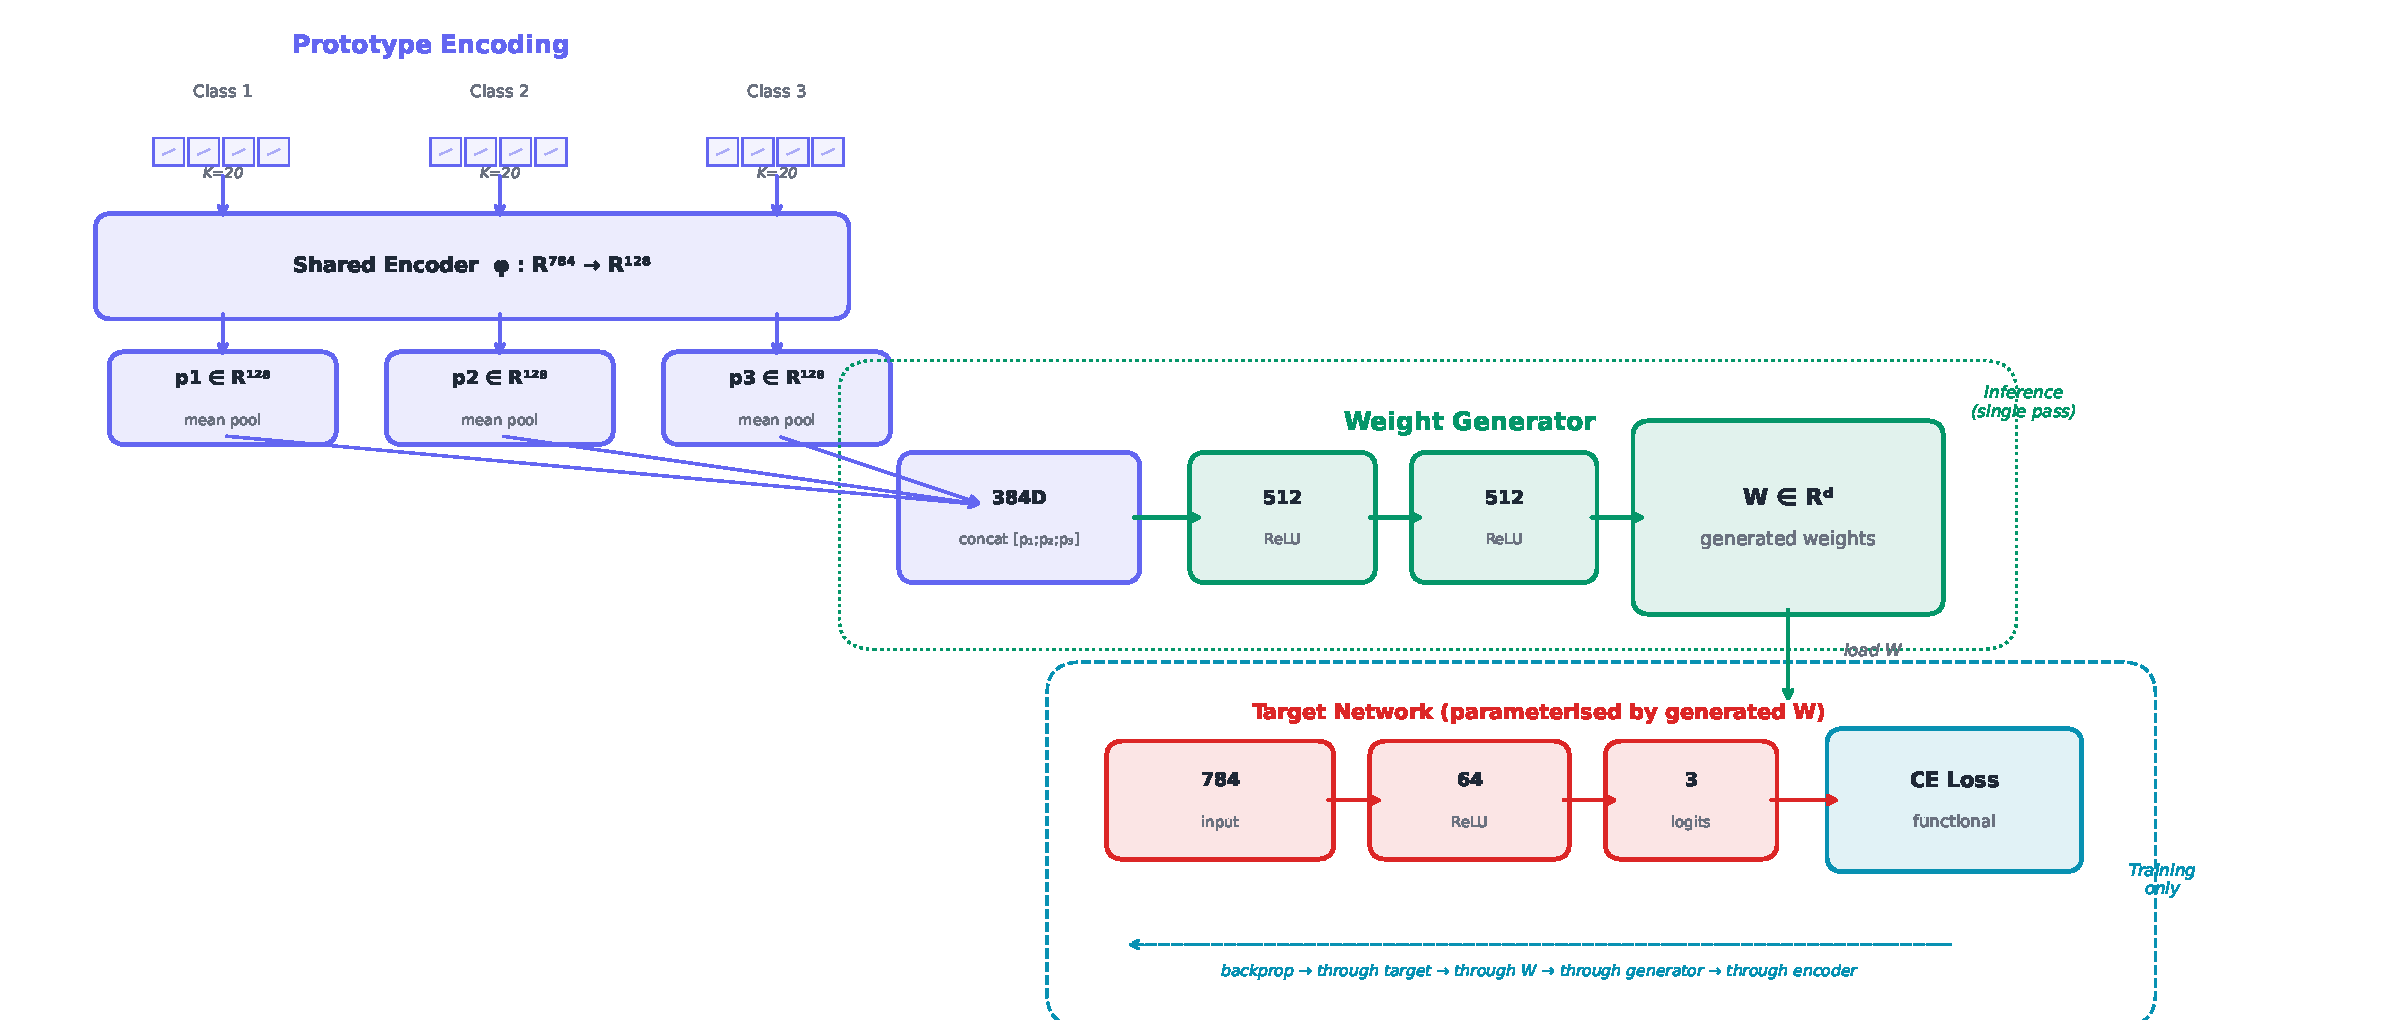
\includegraphics[width=\textwidth]{fig_architecture.pdf}
    \caption{System architecture. \textbf{Top left:} Prototype encoding --- example images from each class are processed by a shared encoder and mean-pooled into 128D prototypes. \textbf{Top right:} Weight generator maps concatenated prototypes to the full target weight vector (green dotted box = inference path, single forward pass). \textbf{Bottom:} During training, generated weights are loaded into the target network and evaluated on task data; the classification loss backpropagates through the entire pipeline (blue dashed box = training only).}
    \label{fig:architecture}
\end{figure}

\subsection{Weight Generation}

\paragraph{Direct generation (50K parameters).}
For targets up to $\sim$50K parameters, an MLP generator maps the task embedding directly to the full weight vector:
\begin{equation}
    W = G(z_{\text{task}}) \in \mathbb{R}^{d}
\end{equation}
The generator has two hidden layers of width 512 with ReLU activations. The target network is a single-hidden-layer MLP ($784 \to 64 \to 3$, $d = 50{,}435$).

\paragraph{SANE-based generation (109K+ parameters).}
Direct generation fails beyond $\sim$50K parameters --- the generated weight vector lands in a flat loss landscape plateau at chance-level performance. We overcome this using SANE tokenisation \cite{schurholt2024towards}: the weight vector is decomposed into per-neuron tokens, each containing one neuron's incoming weights and bias. A Transformer autoencoder learns a compressed latent space over these tokens using functional loss. A latent hypernetwork then maps prototypes to this space, and the frozen decoder reconstructs the full weights. See Section~\ref{sec:sane} for details.

\subsection{Functional Loss}
\label{sec:functional_loss}

The core design decision is \textbf{functional loss}: we train the hypernetwork by \emph{executing} the generated weights as a neural network and backpropagating the classification error:
\begin{equation}
    \mathcal{L}_{\text{func}} = \text{CrossEntropy}\!\left(f(X_{\text{eval}};\; W_{\text{gen}}),\; y_{\text{eval}}\right)
\end{equation}
The forward pass through the target network is implemented as differentiable tensor operations (matrix multiplications using slices of the generated weight vector), enabling gradients to flow from the classification loss through the target network's computations, through the weight values, and back into both the generator and the prototype encoder.

An auxiliary MSE term ($\lambda = 0.1$) provides early-training stability:
\begin{equation}
    \mathcal{L} = \mathcal{L}_{\text{func}} + 0.1 \cdot \mathcal{L}_{\text{MSE}}
\end{equation}

\paragraph{Why functional loss matters.} Weight space contains enormous redundancy: many different weight configurations implement the same function (permutation symmetries, scale invariances, flat directions). MSE treats all weight differences equally; functional loss cares only about differences that affect predictions. As we show in Table~\ref{tab:mse_ablation}, this distinction is not merely quantitative but qualitative: MSE-trained hypernetworks produce initialisations that are \emph{worse} than random, while functional-trained hypernetworks produce \emph{better} ones.

\subsection{SANE Tokenisation for Scaling}
\label{sec:sane}

For target networks beyond 50K parameters, we use a three-stage pipeline:
\begin{enumerate}[noitemsep]
    \item \textbf{Functional autoencoder}: A Transformer encoder-decoder (4 layers, 8 heads, $d_{\text{model}} = 256$) compresses per-neuron weight tokens into a latent space. Trained with functional loss (not MSE) to ensure the latent space preserves weight \emph{function}.
    \item \textbf{Latent hypernetwork}: An MLP maps prototype embeddings to the autoencoder's latent space. Decoder frozen.
    \item \textbf{End-to-end fine-tuning}: Unfreeze decoder, fine-tune the full pipeline with functional loss at reduced learning rate.
\end{enumerate}

% ============================================================
\section{Results}
\label{sec:results}

All results in this section use the \textbf{digits-unseen} split: the system is trained on letter tasks only and evaluated on digit classification tasks where all 3 classes are digits the system has never seen.

\subsection{Core Result: Baselines and Better Minima}

\begin{table}[H]
\centering
\caption{Prototype-conditioned hypernetwork (50K) on all-digit tasks (3/3 unseen classes). The system was trained exclusively on letter tasks. $n = 50$ tasks, paired tests vs each baseline.}
\label{tab:core}
\begin{tabular}{lcccc}
\toprule
\textbf{Initialisation} & \textbf{Zero-shot} & \textbf{+10 FT} & \textbf{+3000 FT} & $\boldsymbol{p}$ \textbf{(vs Generated)} \\
\midrule
\textbf{Generated (ours)} & \textbf{71.6\%} & \textbf{91.8\%} & \textbf{99.3\%} & --- \\
Kaiming He & 33.7\% & 83.7\% & 99.0\% & $10^{-6}$ \\
Random $\mathcal{N}(0, 0.01)$ & 34.0\% & --- & 98.6\% & $< 10^{-6}$ \\
\bottomrule
\end{tabular}
\end{table}

The generated initialisation is already 71.6\% accurate with zero gradient steps --- twice the accuracy of any standard initialisation, which starts at chance (33\%). After 10 fine-tuning steps, the gap remains large: 91.8\% vs 83.7\% for Kaiming. At convergence (3000 steps), the generated initialisation still maintains a statistically significant advantage ($+0.43$pp vs Kaiming, 36/50 wins, $p = 10^{-6}$; $+0.78$pp vs random, 43/50 wins, $p < 10^{-6}$), confirming a genuine \textbf{better-minimum effect}.

\subsection{MAML Comparison}

\begin{table}[H]
\centering
\caption{HyperNet vs MAML vs Kaiming on digit tasks (3/3 unseen). Both MAML and HyperNet trained on letters only. $n = 50$ tasks.}
\label{tab:maml}
\begin{tabular}{rcccc}
\toprule
\textbf{FT Steps} & \textbf{HyperNet} & \textbf{MAML} & \textbf{Kaiming} & \textbf{HN$-$MAML ($p$)} \\
\midrule
0 & \textbf{71.6\%} & 36.1\% & 33.7\% & $+35.5$pp ($< 10^{-6}$) \\
10 & \textbf{91.8\%} & 85.6\% & 83.7\% & $+6.2$pp ($< 10^{-6}$) \\
100 & \textbf{97.6\%} & 96.4\% & 96.2\% & $+1.2$pp ($< 10^{-6}$) \\
3000 & \textbf{99.3\%} & 99.0\% & 99.0\% & $+0.33$pp ($7 \times 10^{-6}$) \\
\bottomrule
\end{tabular}
\end{table}

The hypernetwork outperforms MAML at every fine-tuning budget (all $p < 10^{-5}$). MAML's single shared initialisation, optimised for letter tasks, provides no useful structure for digit classification --- its zero-shot accuracy (36.1\%) is near chance. The hypernetwork's prototype-conditioned generation extracts task-relevant visual features from the digit images and produces an initialisation that is already 71.6\% accurate. At convergence, the hypernetwork still reaches a better minimum ($+0.33$pp, $p = 7 \times 10^{-6}$).

This fundamental difference --- \emph{task-specific} vs \emph{task-agnostic} initialisation --- explains why the hypernetwork generalises across visual domains while MAML does not.

\begin{figure}[H]
    \centering
    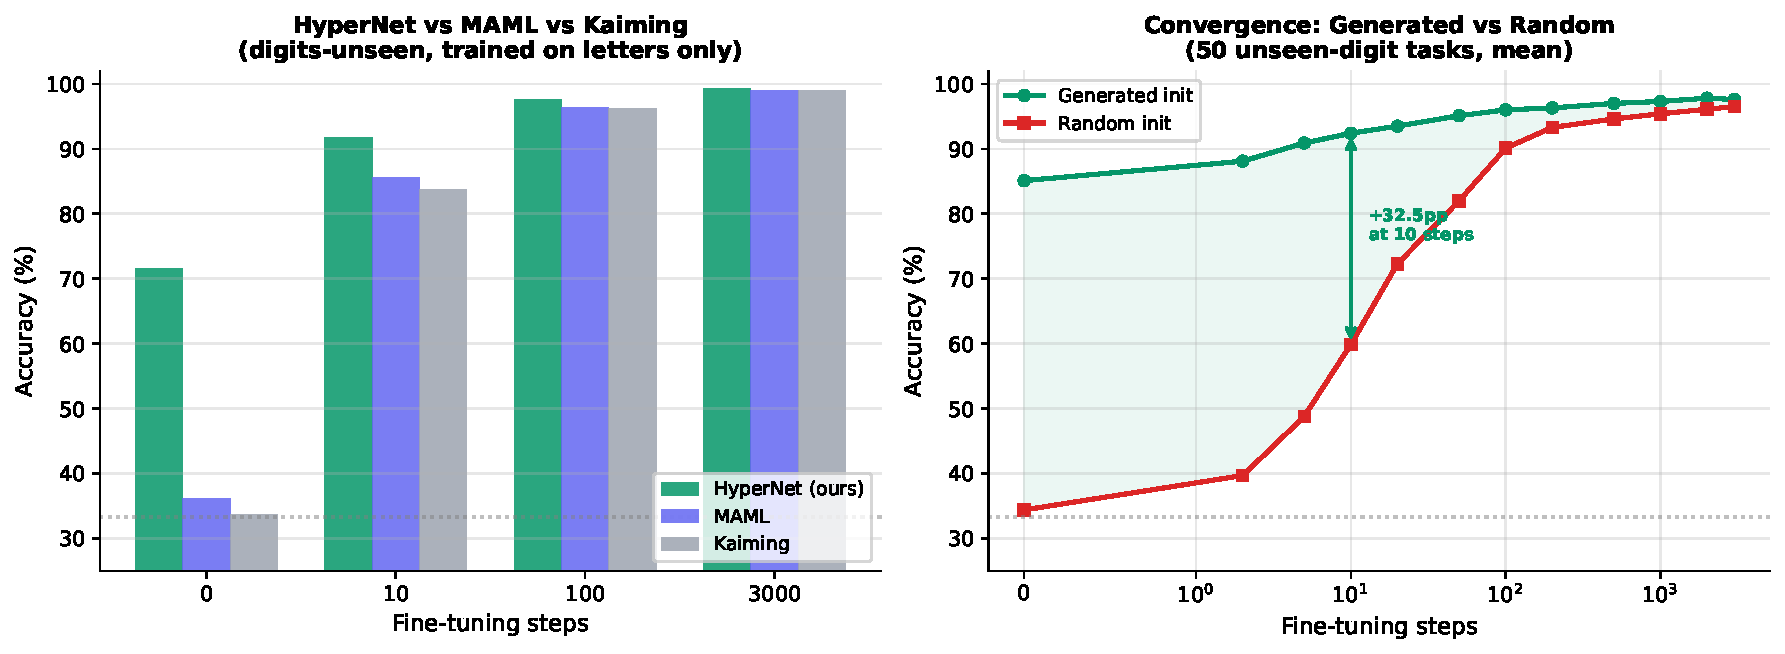
\includegraphics[width=\textwidth]{fig_comparison.pdf}
    \caption{\textbf{Left:} Accuracy comparison at four fine-tuning budgets. The hypernetwork dominates at all budgets, with the largest advantage at 0 steps. \textbf{Right:} Convergence curves for generated vs random initialisation. The shaded area shows the accuracy advantage; the annotation highlights the $+32.5$pp gap at 10 steps. The gap persists at convergence ($+1.1$pp at 3000 steps).}
    \label{fig:comparison}
\end{figure}

\subsection{Convergence Trajectory}

\begin{table}[H]
\centering
\caption{Accuracy over fine-tuning steps, generated vs random initialisation (SGD, 50K, digits-unseen, $n = 50$).}
\label{tab:convergence}
\begin{tabular}{rccc}
\toprule
\textbf{FT Steps} & \textbf{Generated} & \textbf{Random} & \textbf{Gap} \\
\midrule
0 & 85.1\% & 34.4\% & $+50.7$pp \\
10 & 92.4\% & 59.9\% & $+32.5$pp \\
100 & 96.0\% & 90.1\% & $+5.9$pp \\
1000 & 97.3\% & 95.4\% & $+1.9$pp \\
3000 & 97.6\% & 96.5\% & $+1.1$pp \\
\bottomrule
\end{tabular}
\end{table}

The advantage is largest in the low-step regime ($+50.7$pp at step 0, $+32.5$pp at step 10) and persists at convergence ($+1.1$pp at step 3000). The gap narrows but never fully closes. At 3000 steps, generated initialisations win on 41/50 tasks --- the generated weights consistently land in better basins of attraction.

\subsection{Functional vs MSE Ablation}

\begin{table}[H]
\centering
\caption{Loss function ablation (50K, digits-unseen, $n = 50$). Identical hypernetwork architecture and training data; only the loss differs. Functional loss flips the sign of the better-minimum effect.}
\label{tab:mse_ablation}
\begin{tabular}{lcccl}
\toprule
\textbf{Training Loss} & \textbf{Zero-shot} & \textbf{+3000 FT} & \textbf{vs Kaiming} & $\boldsymbol{p}$ \\
\midrule
\textbf{Functional} & \textbf{71.6\%} & \textbf{99.3\%} & $+0.31$pp (33/50) & 0.0001 \\
MSE-only & 33.4\% & 98.5\% & $-0.49$pp (9/50) & 0.00003 \\
Kaiming & 33.7\% & 99.0\% & \multicolumn{2}{c}{\textit{baseline}} \\
\bottomrule
\end{tabular}
\end{table}

This is the cleanest ablation in the paper. Two identical hypernetworks, same architecture, same training data, same prototype encoder --- only the loss function differs:
\begin{itemize}[noitemsep]
    \item \textbf{Functional}: 71.6\% zero-shot, converges to \emph{better} minima than Kaiming ($+0.31$pp, 33/50 wins).
    \item \textbf{MSE-only}: 33.4\% zero-shot (chance), converges to \emph{worse} minima than Kaiming ($-0.49$pp, 9/50 wins).
\end{itemize}

MSE trains the prototype encoder to capture statistical correlations in weight space that are functionally irrelevant. The resulting initialisations not only fail at zero-shot generation but actively mislead gradient descent, producing inferior converged solutions. Functional loss is not merely helpful --- it is \emph{necessary} for the better-minimum effect.

\begin{figure}[H]
    \centering
    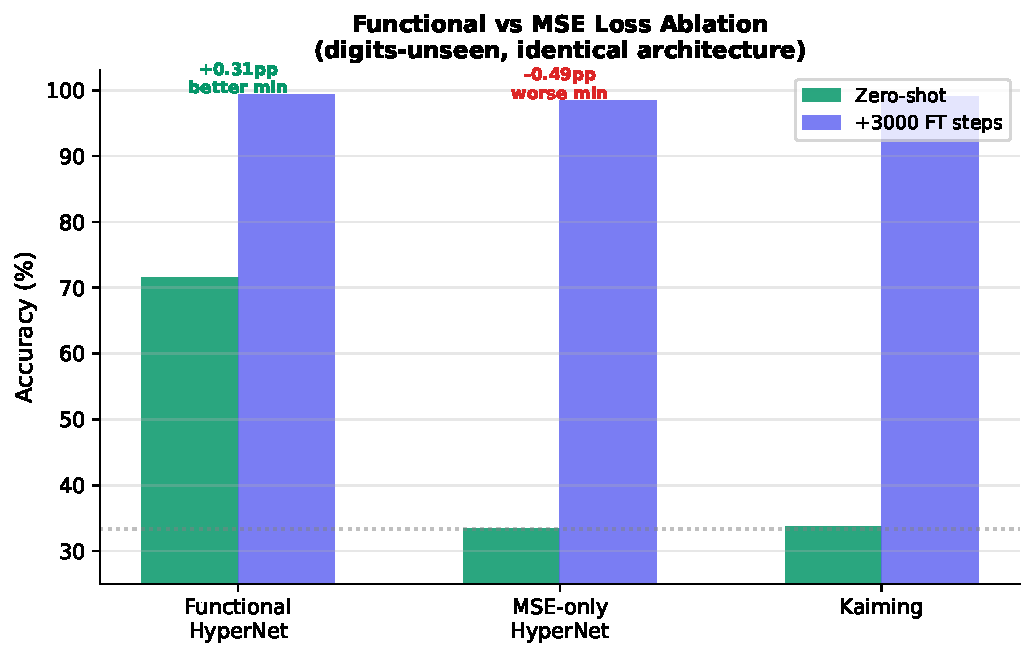
\includegraphics[width=0.55\textwidth]{fig_ablation.pdf}
    \caption{Functional vs MSE loss ablation. Same architecture, same data, same encoder --- only the training loss differs. Functional loss enables 71.6\% zero-shot and converges to a \emph{better} minimum ($+0.31$pp). MSE-only achieves chance-level zero-shot and converges to a \emph{worse} minimum ($-0.49$pp). Functional loss flips the sign of the effect.}
    \label{fig:ablation}
\end{figure}

\subsection{Scaling via SANE (109K Parameters)}

\begin{table}[H]
\centering
\caption{SANE functional generation (109K) with letter-unseen split across novelty levels. 50 tasks per condition, 3000 FT steps.}
\label{tab:sane}
\begin{tabular}{lcccc}
\toprule
\textbf{Unseen Classes} & \textbf{Zero-shot} & \textbf{Gap vs Kaiming} & \textbf{Wins} & $\boldsymbol{p}$ \\
\midrule
0/3 (novel combos) & 88.5\% & $+0.18$pp & 28/50 & 0.017 \\
1/3 & 82.0\% & $+0.32$pp & 34/50 & 0.001 \\
2/3 & 79.1\% & $+0.25$pp & 34/50 & 0.056 \\
\textbf{3/3 (all unseen)} & \textbf{81.4\%} & $\boldsymbol{+0.41}$\textbf{pp} & \textbf{38/50} & $\boldsymbol{0.00006}$ \\
\bottomrule
\end{tabular}
\end{table}

At 109K parameters, direct generation fails (stuck at chance). The SANE-based pipeline overcomes this scaling barrier while preserving the better-minimum effect across all novelty levels. The effect is strongest on fully unseen tasks ($+0.41$pp, $p = 0.00006$), suggesting the system learns generalisable structural priors rather than task-specific solutions.

The SANE functional autoencoder achieves 97\% reconstruction accuracy (vs 33\% for MSE-only), confirming that functional loss is equally critical at the autoencoder level.

% ============================================================
\section{Discussion}
\label{sec:discussion}

\subsection{What the Better-Minimum Effect Means}

The persistent accuracy advantage at convergence ($+0.3$--$0.8$pp after 3000 SGD steps, all $p < 0.001$) indicates that generated weights land in \emph{different, better basins of attraction}. This is confirmed by lower converged cross-entropy loss, not just higher accuracy. The hypernetwork has learned something about the geometry of the loss landscape: which regions contain the best solutions, and how to reach them given visual task descriptions. Figure~\ref{fig:scatter} shows this per-task: the generated initialisation wins on the majority of individual tasks, not just on average.

\begin{figure}[H]
    \centering
    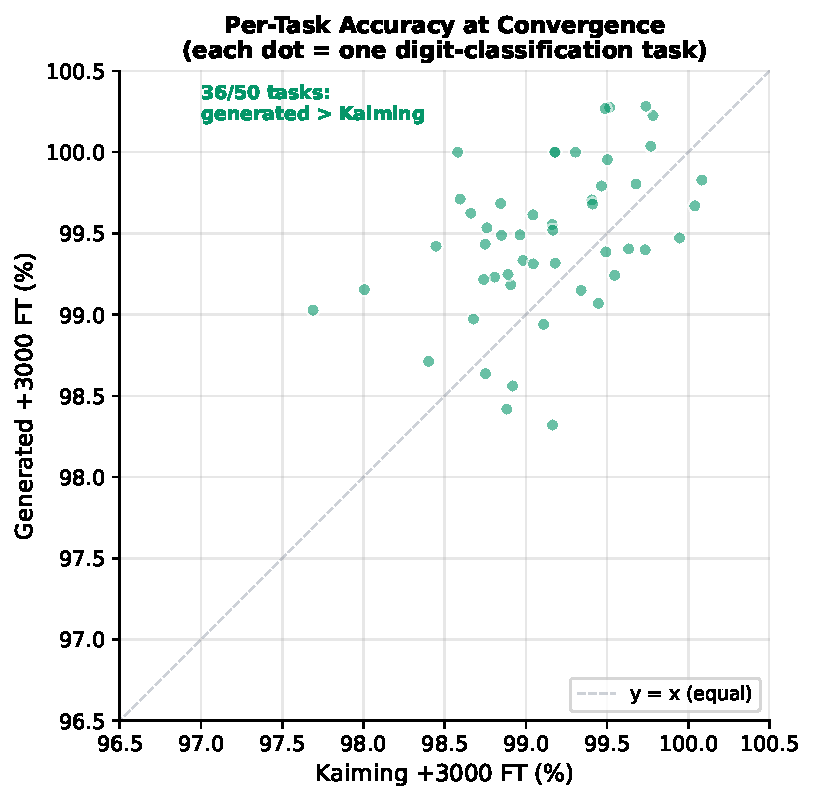
\includegraphics[width=0.5\textwidth]{fig_scatter.pdf}
    \caption{Per-task accuracy at convergence (3000 steps). Each dot is one digit-classification task. Points above the diagonal indicate the generated initialisation converged to higher accuracy. The generated init wins on 36/50 tasks ($p = 10^{-6}$, paired Wilcoxon).}
    \label{fig:scatter}
\end{figure}

\subsection{Why Prototype Conditioning Outperforms MAML}

MAML learns one initialisation $\theta^*$ optimised for the average training task. On unseen domains (digits when trained on letters), this average is useless --- the features it encodes are letter-specific. The hypernetwork avoids this by conditioning on actual test-time images through its shared prototype encoder, which extracts whatever visual structure is available and produces a task-specific initialisation.

\subsection{Limitations}

\begin{itemize}[noitemsep]
    \item The better-minimum effect is small at convergence ($+0.3$--$0.8$pp). The primary practical value is in the low-step regime ($+32$pp at 10 steps).
    \item All experiments use EMNIST (28$\times$28 grayscale). Testing on RGB natural images (CIFAR-100) would further validate the approach.
    \item Target architectures are MLPs. Extension to CNNs via per-channel tokenisation is in progress.
    \item Problem space coverage is just 0.9\% of possible seen-class tasks. Scaling coverage may further improve results.
\end{itemize}

\subsection{Future Work}

\begin{enumerate}[noitemsep]
    \item \textbf{CNN target architectures.} Testing whether the approach generalises from MLP to convolutional weight structures.
    \item \textbf{Problem space coverage scaling law.} Characterising how zero-shot accuracy scales from 1\% to 50\% task coverage.
    \item \textbf{Cross-domain generalisation.} Training on EMNIST, testing on CIFAR-100 or Fashion-MNIST subsets.
    \item \textbf{Continual learning.} Investigating whether the better-minimum effect provides resistance to catastrophic forgetting.
\end{enumerate}

% ============================================================
\section{Conclusion}
\label{sec:conclusion}

We demonstrated that prototype-conditioned hypernetworks, trained with functional loss, generate neural network initialisations that converge to statistically superior local minima compared to standard initialisations (Random, Xavier, Kaiming) and MAML. The effect is verified on tasks where the system must classify digits having been trained exclusively on letters --- a genuine cross-domain test where the prototype encoder has never processed images from the test domain.

Functional loss is the critical design decision. It transforms prototype encoding from a weight-value predictor (MSE, which produces initialisations \emph{worse} than random) into a functional-structure generator (which produces initialisations that find \emph{better} minima). This qualitative flip --- from worse-than-random to better-than-all-baselines --- is the strongest evidence that functional loss enables the hypernetwork to learn meaningful structure about how neural networks solve visual classification tasks.

% ============================================================
\bibliographystyle{plain}
\begin{thebibliography}{9}

\bibitem{finn2017model}
C.~Finn, P.~Abbeel, and S.~Levine.
\newblock Model-agnostic meta-learning for fast adaptation of deep networks.
\newblock In \emph{ICML}, 2017.

\bibitem{snell2017prototypical}
J.~Snell, K.~Swersky, and R.~Zemel.
\newblock Prototypical networks for few-shot learning.
\newblock In \emph{NeurIPS}, 2017.

\bibitem{ha2016hypernetworks}
D.~Ha, A.~Dai, and Q.~V. Le.
\newblock HyperNetworks.
\newblock In \emph{ICLR}, 2017.

\bibitem{schurholt2024towards}
K.~Sch\"{u}rholt, B.~Knyazev, X.~Gir\'{o}-i-Nieto, and D.~Borth.
\newblock Towards scalable and versatile weight space learning.
\newblock In \emph{ICML}, 2024.

\bibitem{cohen2017emnist}
G.~Cohen, S.~Afshar, J.~Tapson, and A.~van Schaik.
\newblock EMNIST: Extending MNIST to handwritten letters.
\newblock In \emph{IJCNN}, 2017.

\end{thebibliography}

% ============================================================
\appendix
\section{Supplementary Ablations}
\label{app:ablations}

This appendix contains additional experiments conducted during development. These use earlier train/test splits (letters as unseen classes, where visual similarity between uppercase and lowercase forms is a confound) and are included for completeness.

\subsection{Letter-Unseen Split (50K, 220 tasks)}

Before adopting the digits-unseen split, we evaluated with seen classes 0--49 and unseen classes 50--61 (lowercase o--z). This split has the weakness that some unseen lowercase letters have visually similar uppercase counterparts in the seen set.

\begin{table}[H]
\centering
\caption{50K direct generation, letter-unseen split, all 3/3 unseen, $n = 220$ tasks.}
\begin{tabular}{lcccc}
\toprule
\textbf{Init} & \textbf{Zero-shot} & \textbf{+3000 FT} & \textbf{Wins} & $\boldsymbol{p}$ \\
\midrule
Generated & 85.1\% & 98.27\% & 174/220 & $<10^{-8}$ \\
Kaiming & 33.3\% & 97.73\% & \multicolumn{2}{c}{\textit{baseline}} \\
Xavier & 33.3\% & 97.01\% & --- & --- \\
Random & 33.3\% & 97.11\% & --- & --- \\
\bottomrule
\end{tabular}
\end{table}

\subsection{Cross-Attention and Task Diversity (50K, Letter-Unseen)}

\begin{table}[H]
\centering
\caption{Ablation of encoder architecture and zoo size (letter-unseen, 50 tasks per variant).}
\begin{tabular}{lcccc}
\toprule
\textbf{Variant} & \textbf{Zero-shot} & \textbf{Gap vs Kaiming} & \textbf{Wins} & $\boldsymbol{p}$ \\
\midrule
A: Mean-pool, 200 tasks & 79.3\% & $+0.54$pp & 36/50 & 0.000004 \\
B: Cross-attention, 200 tasks & 87.2\% & $+0.48$pp & 37/50 & 0.000022 \\
C: Mean-pool, 500 tasks & 89.2\% & $+0.65$pp & 44/50 & 0.000003 \\
D: Cross-attn + 500 tasks & 90.3\% & $+0.68$pp & 43/50 & $< 10^{-6}$ \\
\bottomrule
\end{tabular}
\end{table}

Cross-attention contributes $+7.9$pp zero-shot by modelling inter-class relationships. Task diversity (200$\to$500) contributes $+9.8$pp. The improvements are additive.

\subsection{SANE Scaling to 236K Parameters}

\begin{table}[H]
\centering
\caption{SANE at 236K params (784$\to$256$\to$128$\to$64$\to$3), letter-unseen split.}
\begin{tabular}{lcccc}
\toprule
\textbf{Unseen} & \textbf{Zero-shot} & \textbf{Gap} & \textbf{Wins} & $\boldsymbol{p}$ \\
\midrule
0/3 & 77.2\% & $+0.33$pp & 33/50 & 0.006 \\
1/3 & 65.4\% & $+0.38$pp & 33/50 & 0.002 \\
2/3 & 65.5\% & $+0.24$pp & 27/50 & 0.060 \\
3/3 & 62.0\% & $+0.13$pp & 26/50 & 0.228 \\
\bottomrule
\end{tabular}
\end{table}

The all-unseen effect weakens at 236K ($p = 0.228$), likely due to insufficient zoo size (150 models) relative to target complexity.

\subsection{Functional vs MSE Autoencoder (109K, SANE)}

\begin{table}[H]
\centering
\caption{AE loss ablation for SANE (109K). Recon acc = accuracy of decoded weight vectors.}
\begin{tabular}{lcccc}
\toprule
\textbf{AE Loss} & \textbf{Recon Acc} & \textbf{Zero-shot} & \textbf{Gap vs Kaiming} & \textbf{Better Min?} \\
\midrule
MSE-only & 33\% & 69\% & $-0.46$pp & \textcolor{red}{No} \\
Functional & 97\% & 81\% & $+0.41$pp & \textcolor{green}{Yes} \\
\bottomrule
\end{tabular}
\end{table}

\subsection{Adam vs SGD Optimiser (Letter-Unseen)}

\begin{table}[H]
\centering
\caption{Optimiser comparison at 50K, letter-unseen, $n = 50$.}
\begin{tabular}{lccc}
\toprule
\textbf{Method} & \textbf{+3000 FT} & \textbf{Gap HN$-$Kaiming} & $\boldsymbol{p}$ \\
\midrule
HyperNet + SGD & 98.33\% & $+0.51$pp & 0.00003 \\
HyperNet + Adam & 98.46\% & $+0.18$pp & 0.032 \\
Kaiming + SGD & 97.82\% & \multicolumn{2}{c}{\textit{baseline}} \\
Kaiming + Adam & 98.28\% & \multicolumn{2}{c}{\textit{baseline}} \\
\bottomrule
\end{tabular}
\end{table}

The better-minimum effect holds with Adam ($p = 0.032$) but the gap is smaller because adaptive learning rates partially compensate for suboptimal initialisation.

\end{document}
